\begin{figure}[tb]
	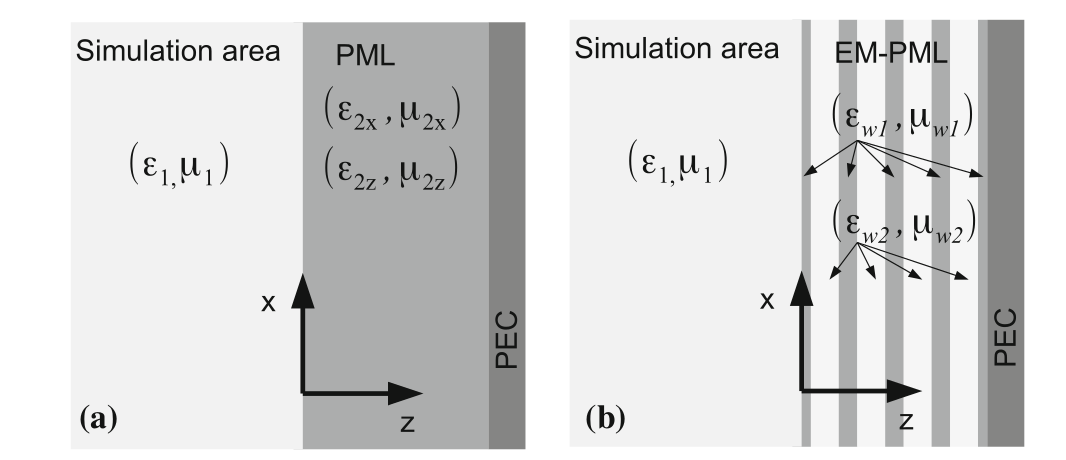
\includegraphics[width=\textwidth]{images/pml/oqe_schemat.png}
	\caption{Schematyczne przedstawienie analizowanej struktury warstwowej i przybliżanego przy pomocy modelu ośrodka efektywnego ośrodka PML}
	\label{fig:pml-multilay-schem}
\end{figure}

Porównując ogólną postać PML podaną w równaniu (\ref{eq:general-pml-form}) z modelem ośrodka efektywnego przedstawionym w podrozdziale \ref{subart:effmedium} można zaproponować przybliżenie ośrodka typu PML przy pomocy struktury warstwowej o odpowiednich właściwościach efektywnych. W szczególności dla uproszczenia analizy skupimy się na polaryzacji TM, dla której istotnymi składowymi tensorów opisujących własności materiałowe są:$\varepsilon_x$,$\mu_y$i $\varepsilon_z$. Ze względu na ograniczenia używanego modelu ośrodka efektywnego, zgodnie ze schmatem na rysunku \ref{fig:pml-multilay-schem} $\varepsilon_x=\varepsilon_y$, oraz $\mu_x=\mu_y$. Ponownie odwołując się do granicy między ośrodkami przedstawione na rysunku \ref{fig:pml-multilay-schem} warunki dla których wielowarstwa będzie efektywnie spełniać rolę PML przedstawiają się następująco:
\begin{equation}
	f\cdot \varepsilon_{w1} + (1-f)\cdot \varepsilon_{w2} = s \cdot \varepsilon_1,
\end{equation}

\begin{equation}
	[f\cdot \varepsilon_{w1}^{-1}+(1-f)\varepsilon_{w2}^{-1}]^-1=s^{-1}\cdot \varepsilon_1,
\end{equation}

\begin{equation}
	f\cdot \mu_{w1} + (1-f)\cdot \mu_{w2} = s \cdot \mu_1,
\end{equation}
gdzie przez $f$ oznaczony został współczynnik wypełnienia, równy ułamkowi przestrzeni wielowarstwy zajmowanemu przez materiał $w1$. Odpowiednie warunki dla polaryzacji TE to:
\begin{equation}
	\varepsilon_{w1}=\rho \frac{\varepsilon_1 \cdot s}{f\cdot \rho + (1 -f) },
	\label{eq:te-eps1}
\end{equation}

\begin{equation}
	\varepsilon_{w2}=\frac{\varepsilon_1 \cdot s}{f\cdot \rho + (1-f)},
	\label{eq:te-eps2}
\end{equation}
gdzie
\begin{equation}
	\rho = 1+\frac{s^2-1 \pm \sqrt{(s^2-1)(s^2-(2f-1)^1)}}{2f(1-f)}.
	\label{eq:te-rho}
\end{equation}

Wykresy na rysunku \ref{fig:upml-eps-s-f} prezentują wyniki obliczonych (\ref{eq:te-eps1}) i (\ref{eq:te-eps2}) jako funkcję współczynnika wypełnienia $f$ i parametru $s$, dla którego przyjęto $s=1+\alpha i$. Używamy rozwiązań dla (\ref{eq:te-rho}) z $|\rho|>1$.




\begin{figure}[tb]
	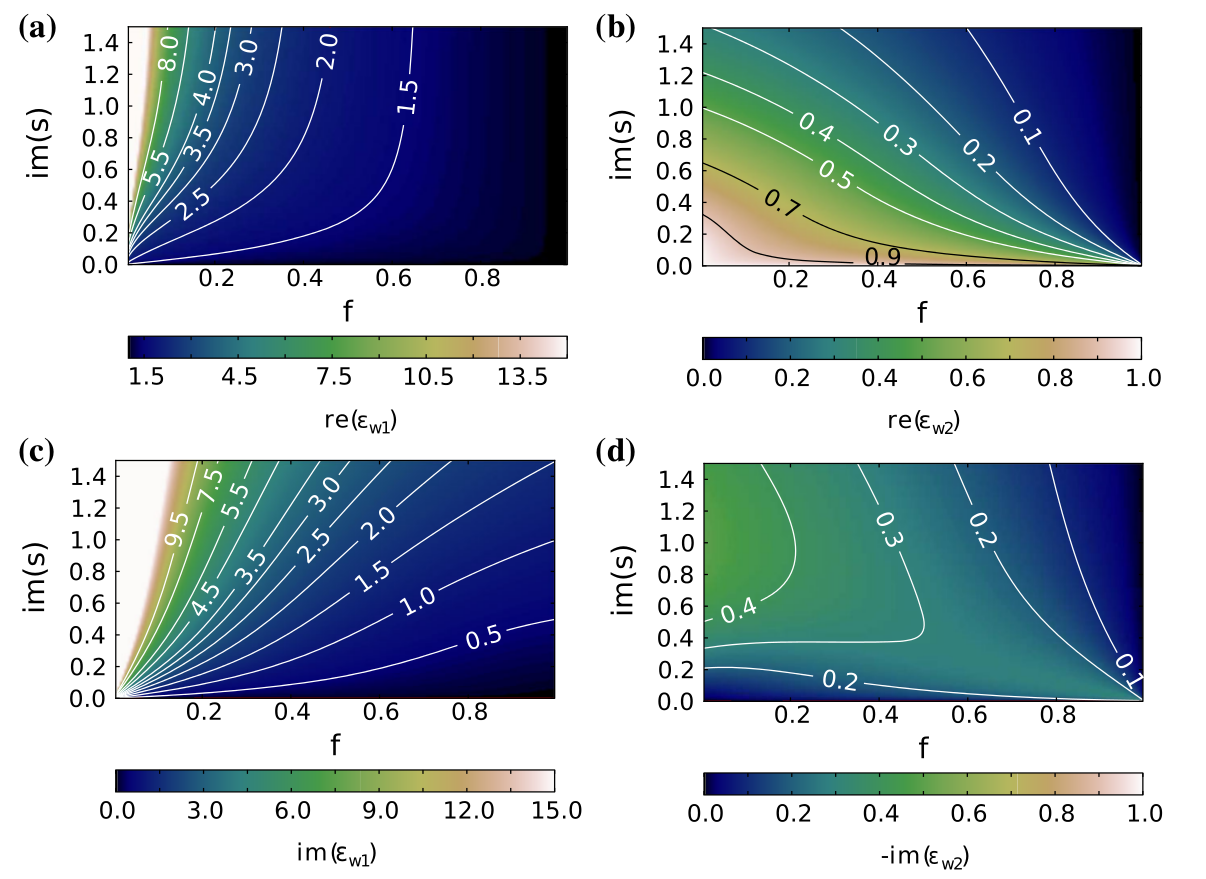
\includegraphics[width=\textwidth]{images/pml/oqe_materials.png}
	\caption{Zależność przenikalności elektrycznej materiałów tworzących UPML (w lewej kolumnie $\varepsilon_{w1}$, w prawej $\varepsilon_{w2}$) w funkcji współczynnika wypełnienia i urojonej części parametru $s$ (założono $\textrm{Re(s)=1}$. Górny wiersz na wykresach (a) i (b) prezentuje zależności części rzeczywistych, dolny na wykresach (c) i (d) części urojonych przenikalności elektrycznych. Ujemne wartości $\varepsilon$ na wykresach (c) i (d) odpowiadają materiałom ze wzmocnieniem optycznym. }
	\label{fig:upml-eps-s-f}
\end{figure}

\begin{figure}[tb]
	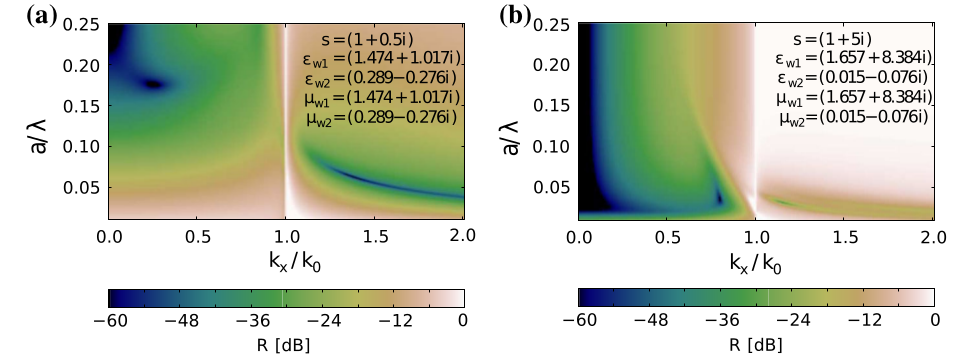
\includegraphics[width=\textwidth]{images/pml/fig3.png}
\end{figure}

\begin{figure}[tb]
	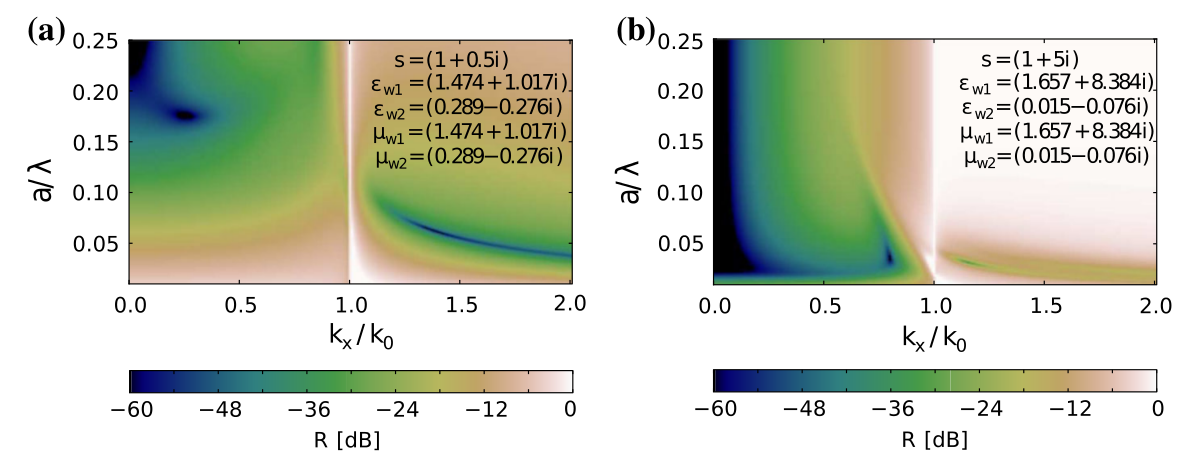
\includegraphics[width=\textwidth]{images/pml/oqe_reflection_kat.png}
\end{figure}

\begin{figure}[tb]
	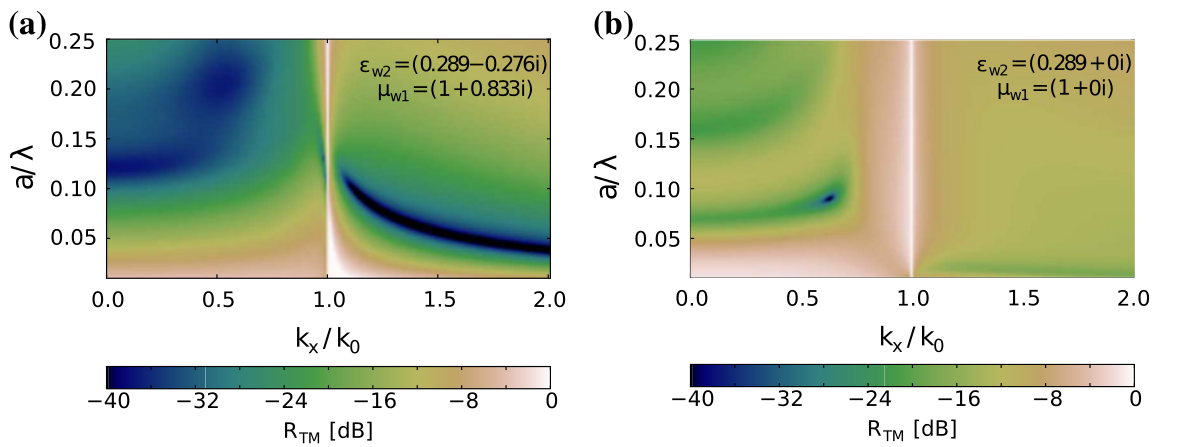
\includegraphics[width=\textwidth]{images/pml/oqe_reflection_kat_simp.png}
\end{figure}

\begin{figure}[tb]
	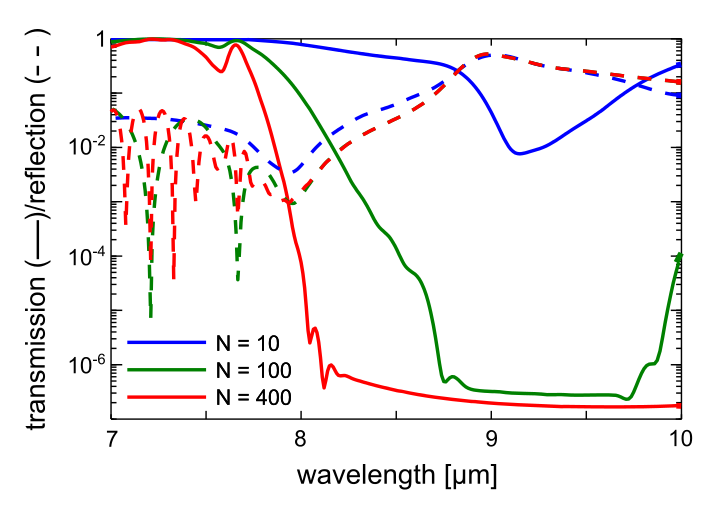
\includegraphics[width=\textwidth]{images/pml/oqe_trans_refl.png}
\end{figure}

\begin{figure}[tb]
	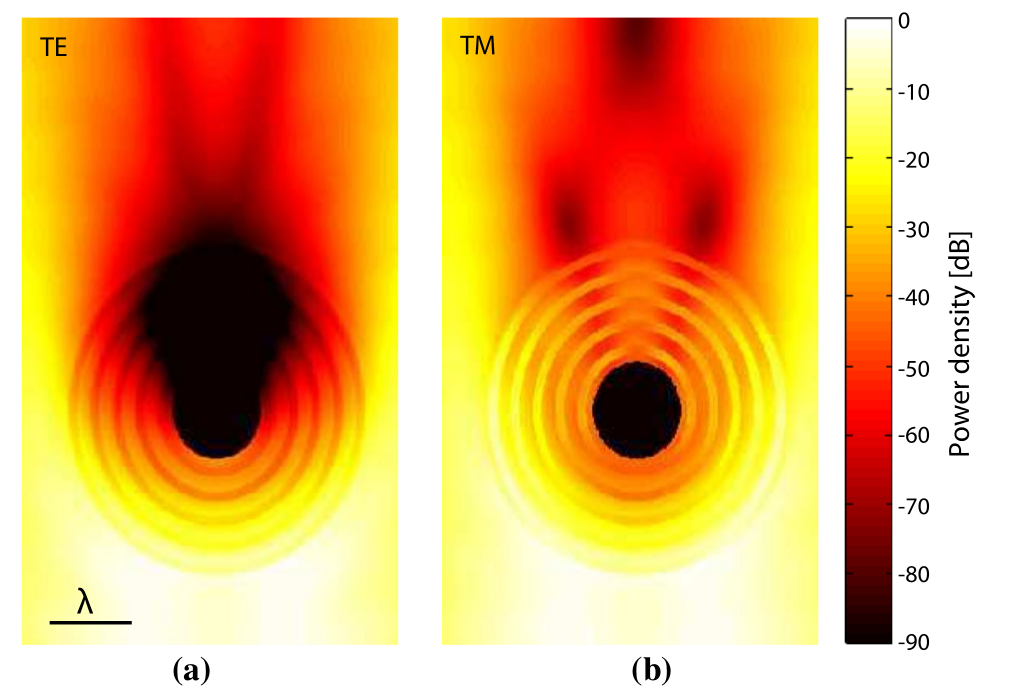
\includegraphics[width=\textwidth]{images/pml/oqe_coreshell.png}
\end{figure}


